\section{User Interfaces}
The user interface is a aspect to distributing a new code base. The interface must be simple but powerful. For SINATRA, the author choose a simple text input file as the base user interface. This combined with a simple execute statement and an accompanying GUI allows for a range of users to use SINATRA to accomplish their tasks. 
\subsection{Running SINATRA}
SINATRA is controlled through a text input file. The developers compile and distribute a new version of SINATRA. This distribution is at it's core a .exe file. Also included is a example text input file. The most basic user only needs to drag the input file onto the .exe file (in Windows\textsuperscript{TM}). They can also just run the executable and input the text input filename, or input it as an argument while running the executable in the command line. An example is shown below.
\begin{verbatim}
    >>DSMC.exe Complex_Input.txt
\end{verbatim}
\indent These multiple options allow the end user to run SINATRA without being caught up in the one specific way of running the program. This ensures that the program will not fall to a classic hereditary code problem where only the original developers are able to run and use the simulation.

\subsection{Input Files}
The input file utilizes a two line system. The first line is a trigger word and the line immediately after it contains the input for SINATRA. The input file is broken into 5 parts. First, is the constant header input. This includes the basic information which includes time step, number density, mesh filename, and velocity. Next is the boundary conditions broken into each of the 6 boundaries. Next is the species information. Then the output files and frequency. Finally is the optional keywords. Each section is split by three stars. This system allows the entire simulation to be compiled once, and complete various tasks just by editing the text file and using it as input. The input file guide can be found in Appendix \ref{app:inputfileguide}. \par
\indent SINATRA is not optimized as a open source and commonly distributed system. It is made to be a Cal Poly homegrown code base. Therefore, it is not built with airtight error checking, complete documentation and support, or perfect distribution and releases. The goal is to have enough of each of those components that competent users in the Cal Poly community may be able to use it to complete simulation and analysis tasks. Therefore, it is possible that there are bugs within the input system in which it will seem that there was no error and that results are displayed, but they are not physical at all. There are error management functions and systems, but they are not foolproof. The user should read previous theses, understand the input file, and have an understanding of DSMC. That being said, it is possible to help the user understand these things simply through a clickable interface. 

\subsection{Graphical User Interface}
The main goal of SINATRA is to be able to simulate rarefied gas for research purposes. It is aimed for use by Faculty, Graduate Students, and specialized Clubs in focused research and projects. However, a DSMC-PIC simulation is a useful tool for even undergraduate classes to test and work with. With that purpose in mind, a Graphical User Interface (GUI) for SINATRA has been created. This GUI is built using MATLAB's Guide tool. It allows a user who has never seen the source code to be able to set up and run simulations. It is built with the expectation that the user does not know how to set up a SINATRA run. The default set up of the GUI can be seen in Figure \ref{fig:SinatraGUI}. \par

\begin{figure}
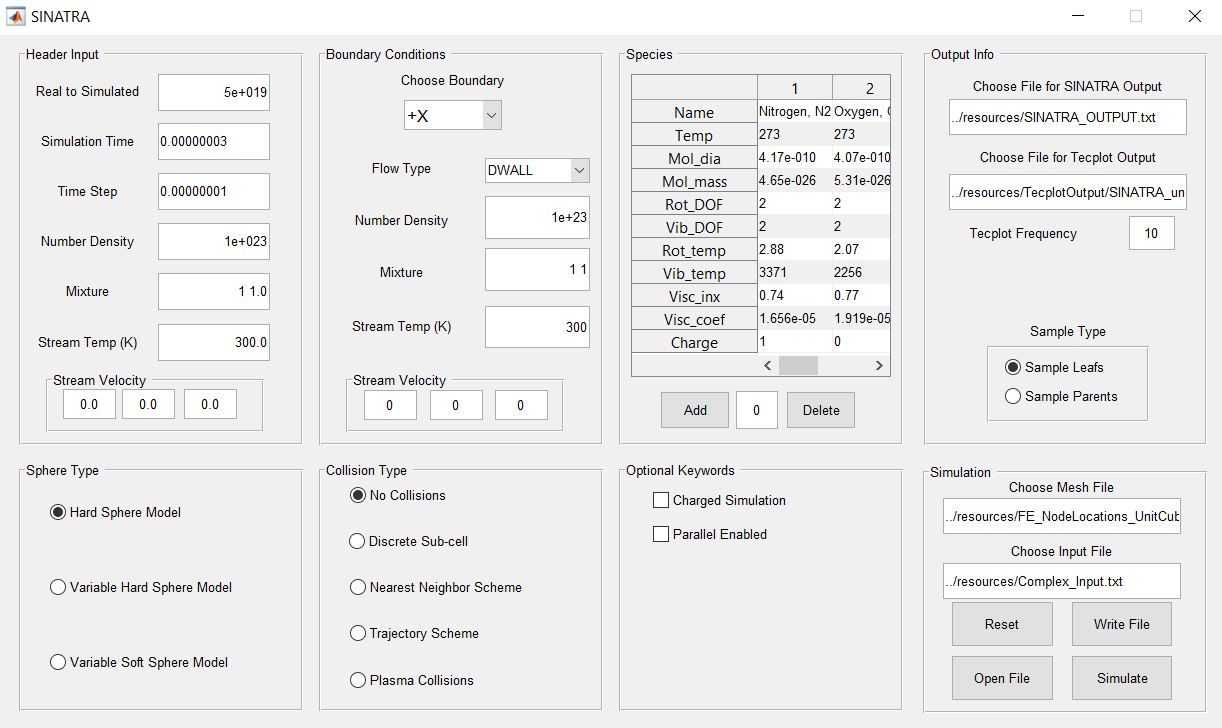
\includegraphics[width=.95\textwidth]{figures/SINATRA_GUI.JPG}
\centering
\caption{Default Setup for SINATRA GUI}
\label{fig:SinatraGUI}
\end{figure}


\indent The GUI allows the user to input the various parameters of a SINATRA run. It does low level error checking on their input to help the user make simulations without many errors. Then the user can create an input text file through a click of a button. The simulation converts the user's inputs into the format of Sinatra's input file. Then the user can select 'Run' and the GUI will takes a current distribution of SINATRA's executable and run it with the recently created input file. The SINATRA GUI is also available as a pure executable, so that the end user does not need to have MATLAB\textsuperscript{TM} installed. 

